
\subsection{Overloading and the Hysteresis Effect}
\label{sxn:hysteresis_effect}

%Here, we do such-and-such. 
%XXX.  HOW PRECISELY TO FRAME.

\michaeladdressed{This par should go somewhere.  Where?}
\charles{@michael: again, no changes to section 6}
Obtaining a value of $\alpha$ outside the $\alpha \gtrsim 2$ range is indicative of ``overloading~\cite{SST92} that layer. 
This can be accomplished, e.g., by training only one layer in the MLP3 model.
As the two layers have very different sizes, we see markedly different behaviors, that are nevertheless consistent with theory.

The \SETOL theory is based on the idea that NNs undergoing training behave like Statistical Mechanic systems relaxing to an equilibrium. 
So far, we have tested the theory under conditions that are approaching \Ideal. 
However, for the theory to be useful in practice, we must also examine how it performs in non-\Ideal situations. 
Of particular interest, we would like to examine the theory under conditions where the training dynamics slows down, i.e., when it is in a ``glassy''
or meta-stable state. 
One way we can do this is to train only one layer, and freeze the rest. 
Doing so overloads the single trainable weight matrix, as a function of the ratio of examples to trainable
parameters~\cite{SST92,Gardner_1988,MM17_TR}, and we expect this to cause $\alpha_{FC1}$ or $\alpha_{FC2}$ to drop well below $2$. As in \ref{sxn:empirical-effective_corr_space}, we will be examining this effect over the entire course of training.

\michaeladdressed{@chris: reorganize the figures in this section, like we discussed.  Also, organie the text properly into each subsubsection.}
\chris{Ive split the figures and re-organized. Lets discuss.}

\subsubsection{Baseline: Loading onto both FC1 and FC2}
\label{sxn:hysteresis_baseline}
\begin{figure}[t] %[h]
    \centering
%    \subfigure[FC1 \ALPHA vs train and test error]{
        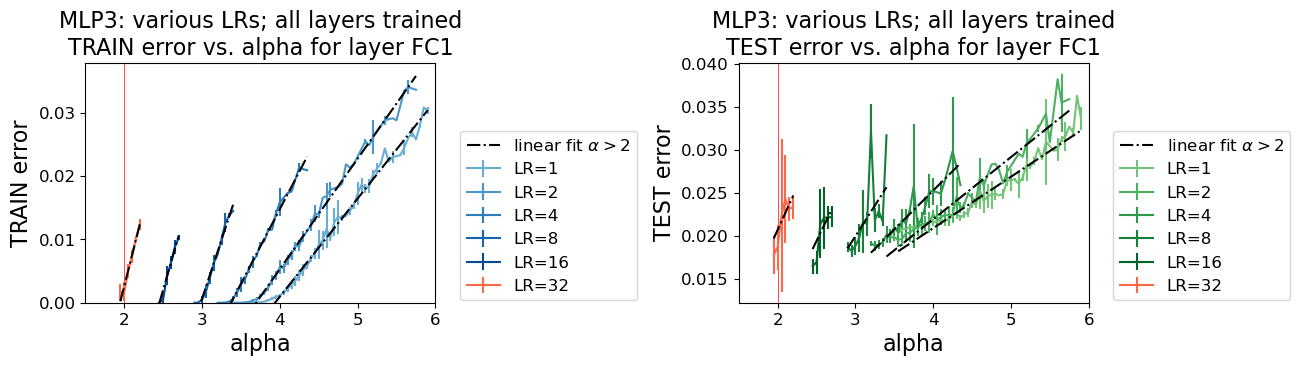
\includegraphics[width=15cm]{img/alpha_by_scales/mlp3_error_by_LR_all_FC1_binned.png} \\
%        \label{fig:mlp3-FC1-alpha-all-trained}
%    }\\
    \begin{tabular}{ccc}
      (a)\hspace{5cm} & (b) 
    \end{tabular}
%    \subfigure[FC2 \ALPHA vs train and test error]{
        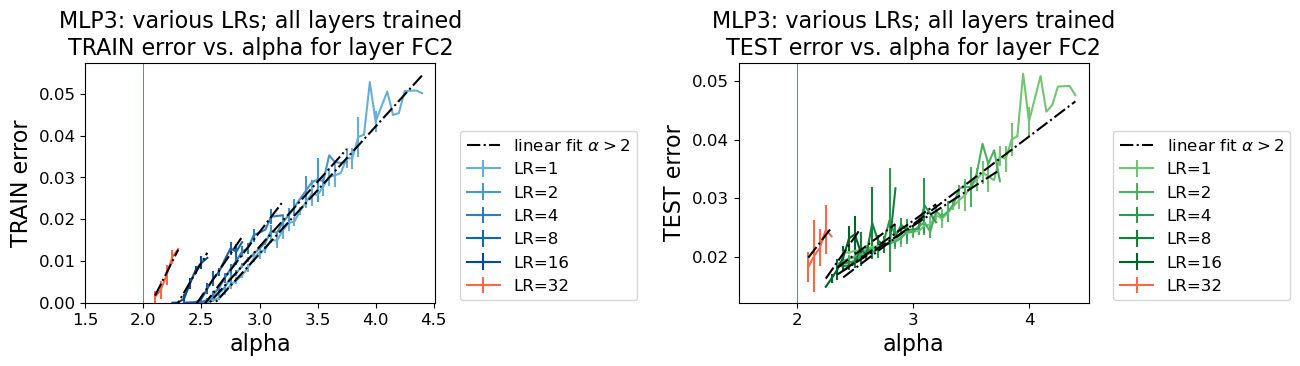
\includegraphics[width=15cm]{img/alpha_by_scales/mlp3_error_by_LR_all_FC2_binned.png}
%        \label{fig:mlp3-hyst-all-FC2-LR32}
%    }
    \begin{tabular}{ccc}
      (c)\hspace{5cm} & (d) \\
    \end{tabular}
    \caption{
        Train (a, c) and test (b, d) accuracy as a function of $\alpha_{FC1}$ (a, b) and $\alpha_{FC2}$ (c, d) when {\bf all 
        layers are trained}. Red vertical lines show the critical value of $\alpha = 2$, and dashed black lines show 
        linear fits of error, using only points where $\alpha > 2$ and train error $> 0.001$. 
        For FC1 (a, b), we can see that each learning rate 
        produces a different trajectory of train error (a) and test error (b) as a function of $\alpha_{FC1}$, 
        showing that even though FC1 dominates overall, (Table~\ref{tab:mlp3},) FC2 still plays a modulating role. 
        (Cf. Figure~\ref{fig:mlp3-FC1-alpha-overloaded} where there is only one trajectory.)
        In (c, d) we can see that $\alpha_{FC2}$ never goes below $2$. As in (a, b), each learning rate 
        produces a different trajectory, though there is greater overlap for lower learning rates. See discussion in 
        Section~\ref{sxn:hysteresis_baseline}.
    }
    \label{fig:mlp3-baseline-load}
\end{figure}


%\michaeladdressed{Backpoint explicitly to what figs/section is being referred to here.} Done

To start, Figure~\ref{fig:mlp3-baseline-load} shows $\alpha_{FC1}$ and $\alpha_{FC2}$, binned in units of $0.05$, versus 
train and test error over all epochs of training
\footnote{Excluding the first four epochs when the matrix is still essentially random.} 
for each of the different learning rates considered. 
(Cf. Figures~\ref{fig:mlp3-alphas-lr} and~\ref{fig:mlp3-alphas-bs}, Section~\ref{sxn:empirical-effective_corr_space},
which show only the final epoch.)
Binning was done so as to facilitate averaging over the $5$ starting random seeds; 
linear fits are shown separately for each learning rate; and
error bars represent one standard deviation within each bin. 
The critical value of $\alpha=2$ is shown as a vertical red line in all plots. 
For each learning rate, train error and $\alpha$ decrease together during training, which can be seen for both 
$\alpha_{FC1}$ (a) and $\alpha_{FC2}$ (c), reading each line from the top right to bottom left. Test errors, (b, d) show 
a similar trend, but with wider error bars. 
Observe that the range of the y-axis is narrower for test error to make detail more visible.
\chris{CH TODO: Double check these plots. The y-axis should be the same vertically.}

We see in Figure~\ref{fig:mlp3-baseline-load} (a,b) 
\michaeladdressed{soft-code, dont hard-code subfigure references}
\chris{Splitting these figures is manual, so the soft-coding is a stand-in until they are finalized and frozen.}
that the $32\times$ learning rate causes $\alpha_{FC1}$ to decrease faster than any other, putting it on course to 
fall below $2$ before train error reaches $\simeq 0$. 
(See Figure~\ref{fig:mlp3-accuracies}, at the beginning of this Section.) 
We also see that the slower learning rates cause train error to reach $\simeq 0$ well before $\alpha_{FC1}$ can reach $2$, and this offers an explanation as to why their test error was higher.

%the FC1 layer, which has been shown to dominate 
%learning -- test error behaves more concordantly with FC1 $\alpha_{FC1}$. With FC1 frozen to its initial random state, the 
%much smaller FC2 will have to do all of the learning. 


\subsubsection{Overloading FC1}
\label{sxn:hysteresis_effect_FC1}


\begin{figure}[t] %[h]
    \centering
%    \subfigure[FC1 \ALPHA vs train and test error]{
        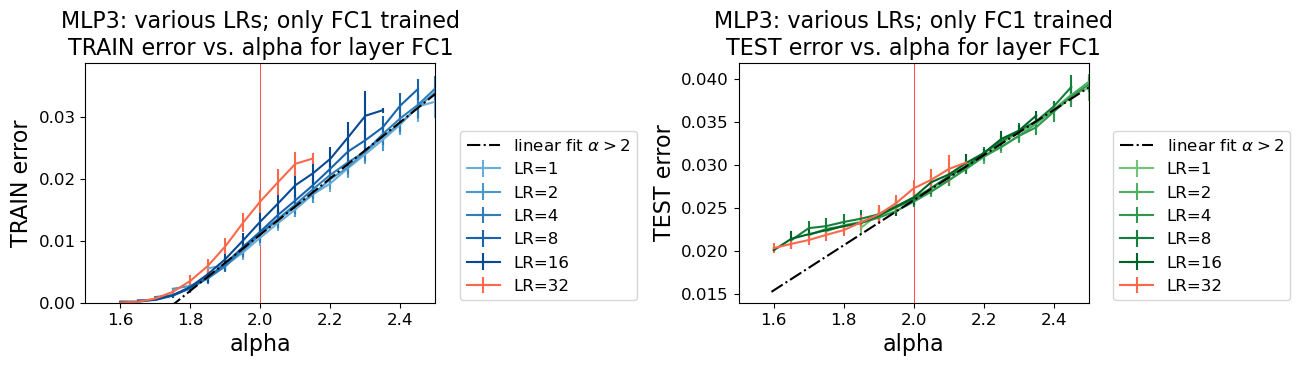
\includegraphics[width=15cm]{img/alpha_by_scales/mlp3_error_by_LR_FC1_FC1_binned.png}
%        \label{fig:mlp3-FC1-alpha-FC1-trained}
%    }
    \begin{tabular}{ccc}
      (a)\hspace{5cm} & (b) \\
    \end{tabular}
    \caption{
            Train and test accuracy as a function of $\alpha_{FC1}$ when only FC1 is trained (a, b). 
            Red vertical lines show the critical value of $\alpha_{FC1} = 2$, and dashed black lines show 
            linear fits of error, using only points where $\alpha_{FC1} > 2$. 
            In contrast with Figure~\ref{fig:mlp3-baseline-load}, when only 
            FC1 is trained, we can see that no matter the learning rate, there is ony one trajectory, for both train 
            error (a) and test error (b). Hence, for visibility, only one linear fit, using all learning rates pooled, 
            is shown. Crucially, we can see in (b) that as $\alpha_{FC1}$ passes below $2$, the \emph{test error} 
            trajectory changes, for all learning rates, even as the \emph{train error} trajectory does not, until it 
            reaches $\sim 0$. This suggests that even though test accuracy can still decrease when $\alpha_{FC1} < 2$, it 
            does so at a decreased rate relative to $\alpha_{FC1}$. See discussion in 
            Section~\ref{sxn:hysteresis_effect_FC1}.
    }
    \label{fig:mlp3-FC1-alpha-overloaded}
\end{figure}


In contrast, when only FC1 is trained, Figure~\ref{fig:mlp3-FC1-alpha-overloaded} shows that, as expected, 
$\alpha_{FC1}$ decreases well below $2$. Training error (a) generally trends downward as $\alpha_{FC1}$ decreases, 
but no matter the learning rate, the relation is the same, or nearly so, because only one layer is being trained. 
Consequently, all learning rates were pooled to produce one linear fit for enhanced visibility.

In Figure~\ref{fig:mlp3-FC1-alpha-overloaded} we can see 
demonstration of a crucial claim of \SETOL theory: that for $\alpha_{FC1} > 2$, (vertical red line,) the test 
error declines linearly; (b) shows that test error is almost perfectly linear with decline in $\alpha_{FC1}$. However, when $\alpha_{FC1} < 2$, the curve bends 
upward. 
Furthermore, the precision with which the trajectory changes as $\alpha_{FC1}$ passes the threshold provides ample 
validation that the estimator of~\cite{CSN09_powerlaw} is indeed accurate. We 
observe that test error may continue to decrease after $\alpha_{FC1} < 2$, however the rate of decrease is significantly less. 
We can also see that in some sense, the model is ``doomed'' to always have train error reach $\simeq 0$ when 
$\alpha_{FC1} \simeq 1.7$, i.e., after $\alpha = 2$, because of the number of trainable parameters, and perhaps because 
of the lack of a modulating influence of FC2 seen in Figure~\ref{fig:mlp3-baseline-load}.

\chris{This might be a good place to cite Temperature Balancing, Layer-wise Weight Analysis, and Neural Network Training because this corroborates the idea that learning rates work differently on different layers.}\michael{Yes.}
\charles{@michael: do it then!}


%In the FC1 layer we see that as $\alpha$ decreases below $2$, the rate of 
%decrease of test error begins to slow down at exactly that point. In FC2, which has much less capacity for storing 
%patterns, we see a different behavior resembling a Hysteresis curve\cite{???}. We also observe a point beyond which the 
%different random seeds show markedly different behavior which we conjecture is a result of \Replica Symmetry 
%Breaking\cite{SST92}.


\subsubsection{Overloading FC2}
\label{sxn:hysteresis_effect_FC2}

\begin{figure}[t] %[h]
    \centering
%    \subfigure[FC2 \ALPHA \LearningRate $16\times$]{
        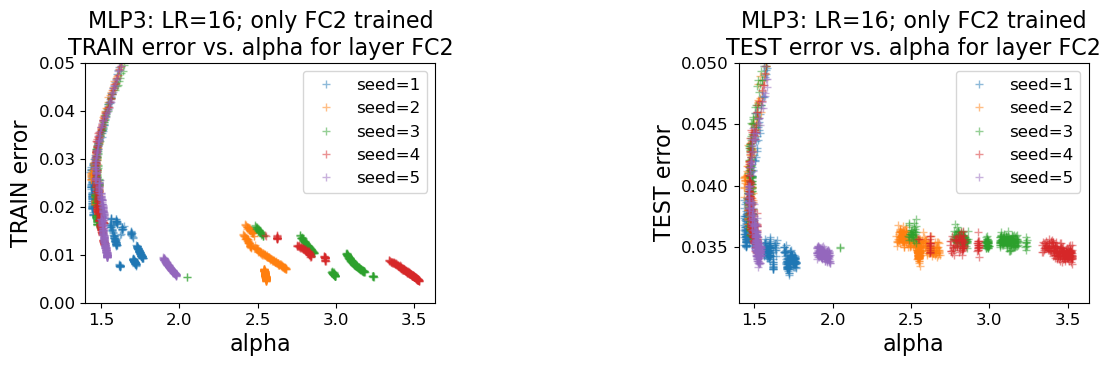
\includegraphics[width=15cm]{img/alpha_by_epochs/mlp3_error_by_LR=16_FC2_FC2.png}
%        \label{fig:mlp3-hyst-FC2-FC2-LR16}
%    }\\
    \begin{tabular}{ccc}
      (a)\hspace{5cm} & (b) \\
    \end{tabular}
%    \subfigure[FC2 \ALPHA \LearningRate $32\times$]{
        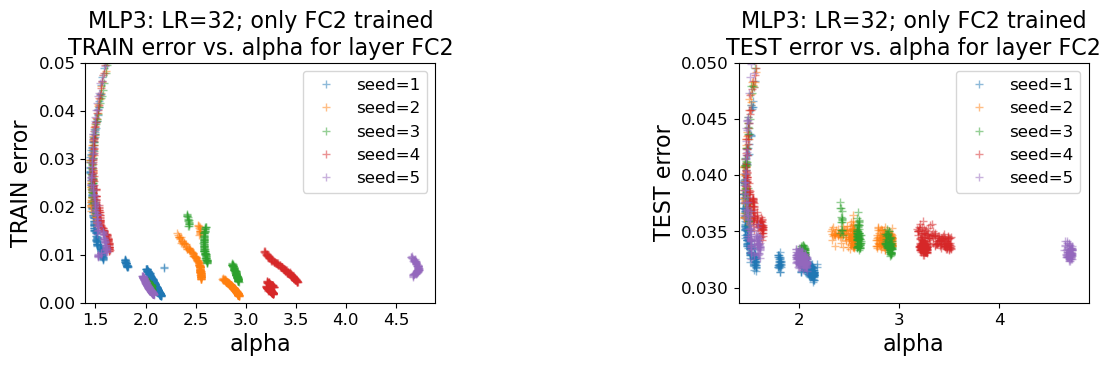
\includegraphics[width=15cm]{img/alpha_by_epochs/mlp3_error_by_LR=32_FC2_FC2.png}
%        \label{fig:mlp3-hyst-FC2-FC2-LR32}
%    }
    \begin{tabular}{ccc}
      (c)\hspace{5cm} & (d) \\
    \end{tabular}
        \caption{Train error (a, c) and test error (b, d) as a function of $\alpha_{FC2}$ when all other layers are 
        frozen, for the two largest learning rates, $lr=16\times$, (a, b) and $lr=32\times$(c, d). Cf. 
        Figure~\ref{fig:mlp3-baseline-load}, wherein all layers were trained. Due to the markedly different 
        behavior of each random seed, they cannot be plotted as means and error bars, and are instead shown separately. 
        The path taken by all seeds up to $\alpha_{FC2} = 1.5$ has a slight curvature characteristic of a 
        hysteresis-like behavior. Observe also that the fragmenting into separate paths, due to the breakdown of the 
        PL tail, coincides roughly with each seeds path reaching its minimum test error. The y-axis is scaled 
        differently for train and test error to make variation more visible. See discussion in 
        Section~\ref{sxn:hysteresis_effect_FC2}.
    }
    \label{fig:mlp3-FC2-alpha-hysteresis}
\end{figure}

\michaeladdressed{This par maybe should go into the baseline subsection above.}
\chris{See my changes.}
The MNIST dataset has $60,000$ training examples, which means that an FC1-only model is over-parameterized, but FC2 is 
substantially \emph{under}-parameterized~\cite{DLM19_Exact_TR}. (Table~\ref{tab:mlp3}) This drastically changes the 
meaning of an experiment where only FC2 is trained. Figure~\ref{fig:mlp3-baseline-load} (Section 
\ref{sxn:hysteresis_baseline}) shows $\alpha_{FC2}$ vs. train error (c) and test error (d) when \emph{all} layers are 
trained. There we see a different relationship between $\alpha_{FC2}$ and train and test error for each learning rate. 
None of the training runs reached an $\alpha_{FC2}$ of $2$, as the load was split between both layers FC1 and FC2.

Figure~\ref{fig:mlp3-FC2-alpha-hysteresis}, however, shows a starkly different relationship. 
\michaeladdressed{We need to show more, especially earlier in training, so its clear that the curves are similar and then split.}
\charles{@michael: Chris has moved on and we need to work with what we have}
When only FC2 is trained, 
each random seed produces a different trajectory, meaning that they cannot be interpretably plotted as a single curve, even with error 
bars. Train (a, c) and test (b, d) error rates are shown as a function of $\alpha_{FC2}$ for the two highest learning 
rate factors, $16\times$ (a, b) and $32\times$ (c, d). Lower learning rate factors, (not shown,) showed the same trend, except 
that they did not progress as far as those shown in Figure~\ref{fig:mlp3-FC2-alpha-hysteresis}.
\michaeladdressed{Not clear.}
\charles{@michael: this should have been addressed a year ago}

First we see, for all seeds, $\alpha_{FC2}$ decreases all the way down to $1.5$, after which it begins to rebound to the 
right. As it 
does, train error continues to decrease. We can also see that test error continues to decrease as well, down to its minimum 
value of slightly more than $0.03$, as $\alpha_{FC2}$ continues to increase for a short time. However, at the exact 
point where test error reaches a minimum, the PL tail itself begins to fracture, leading to different estimates 
of $\alpha_{FC2}$ for each seed. As each of the five starting random seeds are shown separately, we can see that each of 
them terminates at a different point, some of which are closer to $2$ than others.

Such a reversion to a more \Typical value of $\alpha_{FC2}$, prior to the fracturing of the PL tail, is 
reminiscent of a spin glass system relaxing towards its minimum energy configuration, in a way that retains some memory 
of the path taken on the way to its current state. 
\michaeladdressed{We show fracturing, then claim it is \ATypical, but we dont show hysterisis, which is the title of the subsection.  We should show that explicitly to be more clear.}
\chris{The claim of hysteresis is based on the bending seen in the curve (left, top to bottom,) just before fracturing 
        happens. We can also see that though the curves fracture, they all continue bending strongly to the right.
        The theory predicts that alpha will decrease, but it doesnt predict that it will rebound as we see there. The 
        only mechanism we know of that would predict such bending, seen most clearly in (a, c), is hysteresis.
}
We conjecture that if the model were trained for sufficiently many 
epochs, (perhaps many thousands,) then the tail would re-form, and $\alpha_{FC2}$ would reform, and revert all the way back to its 
stable value of $2$.

